\section{Experiments}

\begin{frame}
\frametitle{Experimental Results: Comparison with SOTA}
\begin{itemize}
    \item Key metrics maintain high levels across multiple datasets
    \begin{columns}[T]
    \column{0.3\textwidth}
    \begin{figure}[H]
        \centering
        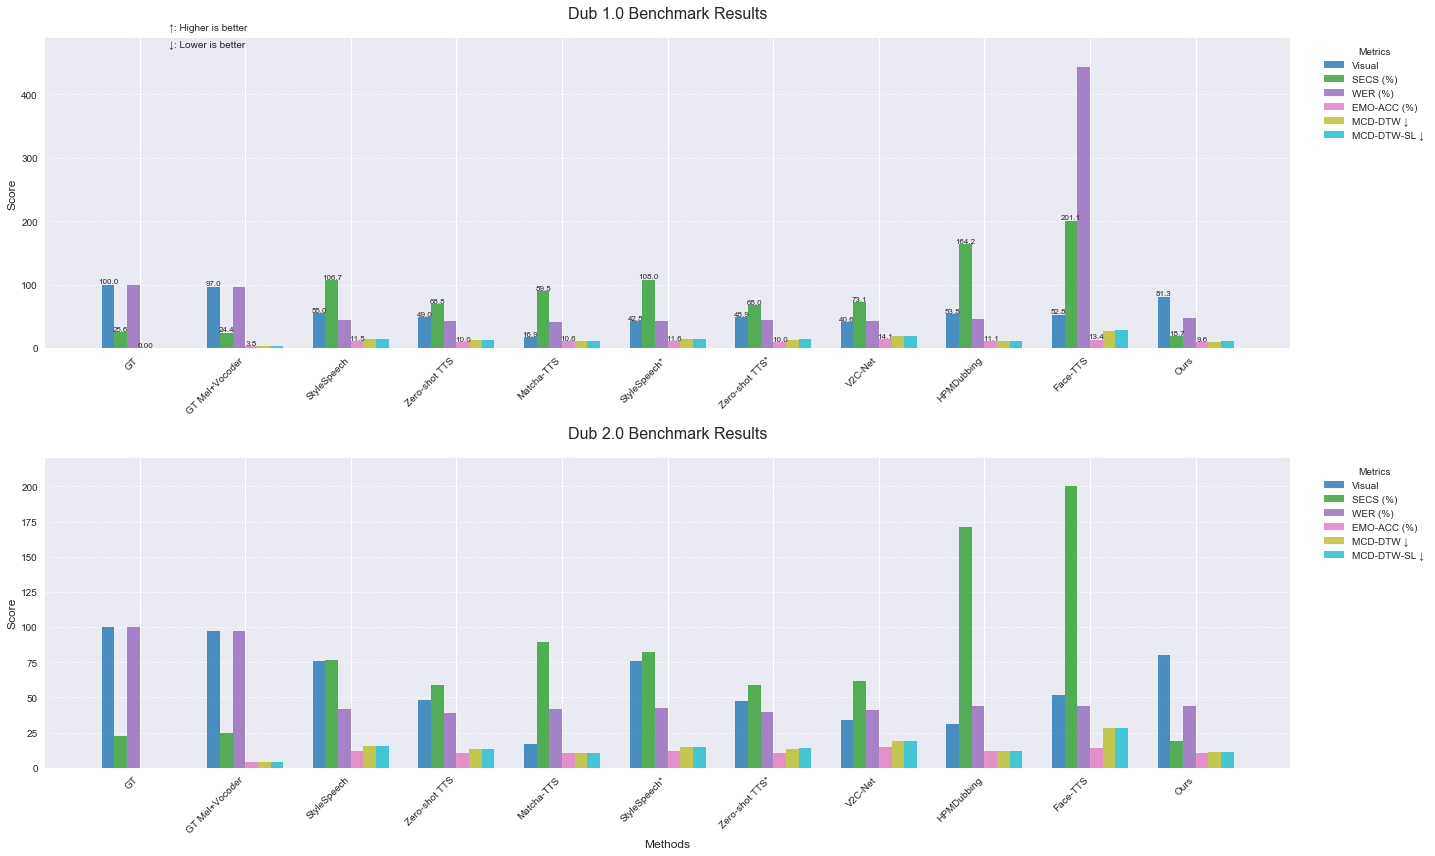
\includegraphics[width=\linewidth]{figs/1table.png} % Replace with the image path for V2C-Animation dataset results
        \caption{V2C-A Dataset Test Results}
        \label{fig:v2c-animation}
    \end{figure}

    \column{0.3\textwidth}
    \begin{figure}[H]
        \centering
        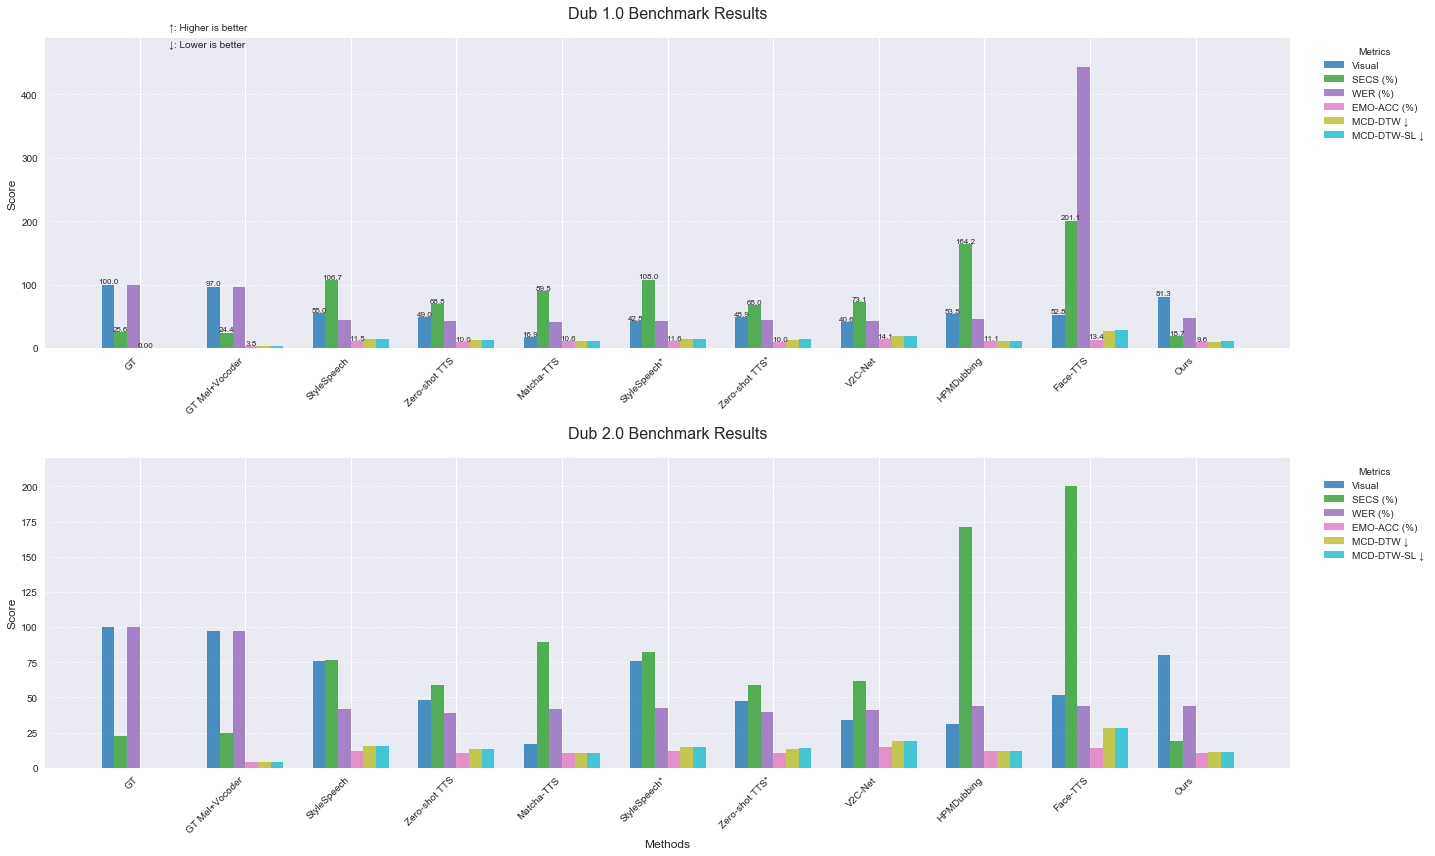
\includegraphics[width=\linewidth]{figs/1table.png} % Replace with the image path for GRID dataset results
        \caption{GRID Dataset Test Results}
        \label{fig:grid}
    \end{figure}
\end{columns}

\begin{columns}[T]
    \column{0.3\textwidth}
    \begin{figure}[H]
        \centering
        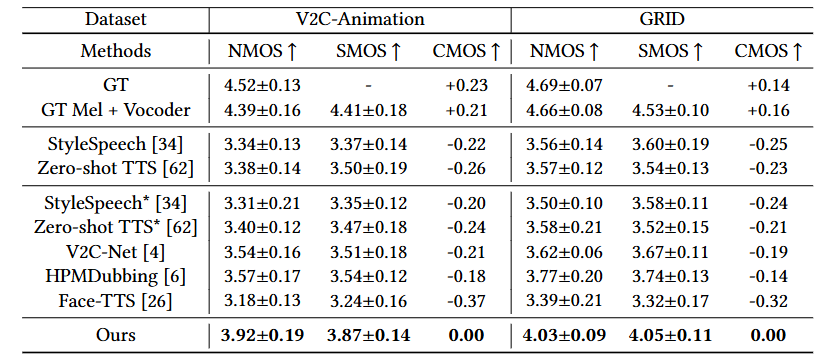
\includegraphics[width=\linewidth]{figs/table3.png} % Replace with the image path for zero-shot test results
        \caption{Zero-shot Test}
        \label{fig:zeroshot}
    \end{figure}

    \column{0.3\textwidth}
    \begin{figure}[H]
        \centering
        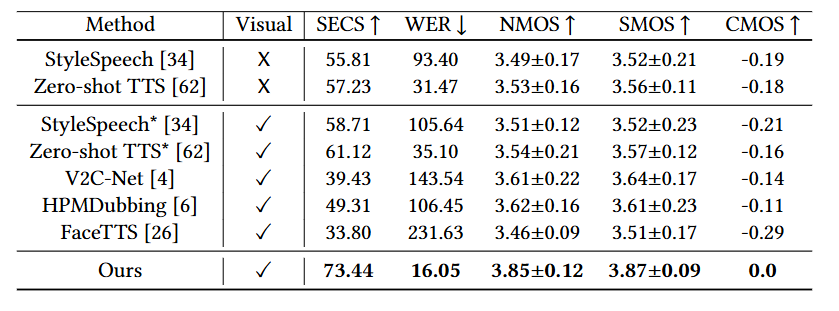
\includegraphics[width=\linewidth]{figs/table4.png} % Replace with the image path for subjective evaluation results
        \caption{Subjective Evaluation Results}
        \label{fig:subjective}
    \end{figure}
\end{columns}
\end{itemize}
\end{frame}


% \begin{frame}
% \frametitle{Experimental Results: Qualitative Analysis of Mel Spectrograms}
% \begin{figure}
% \centering
% 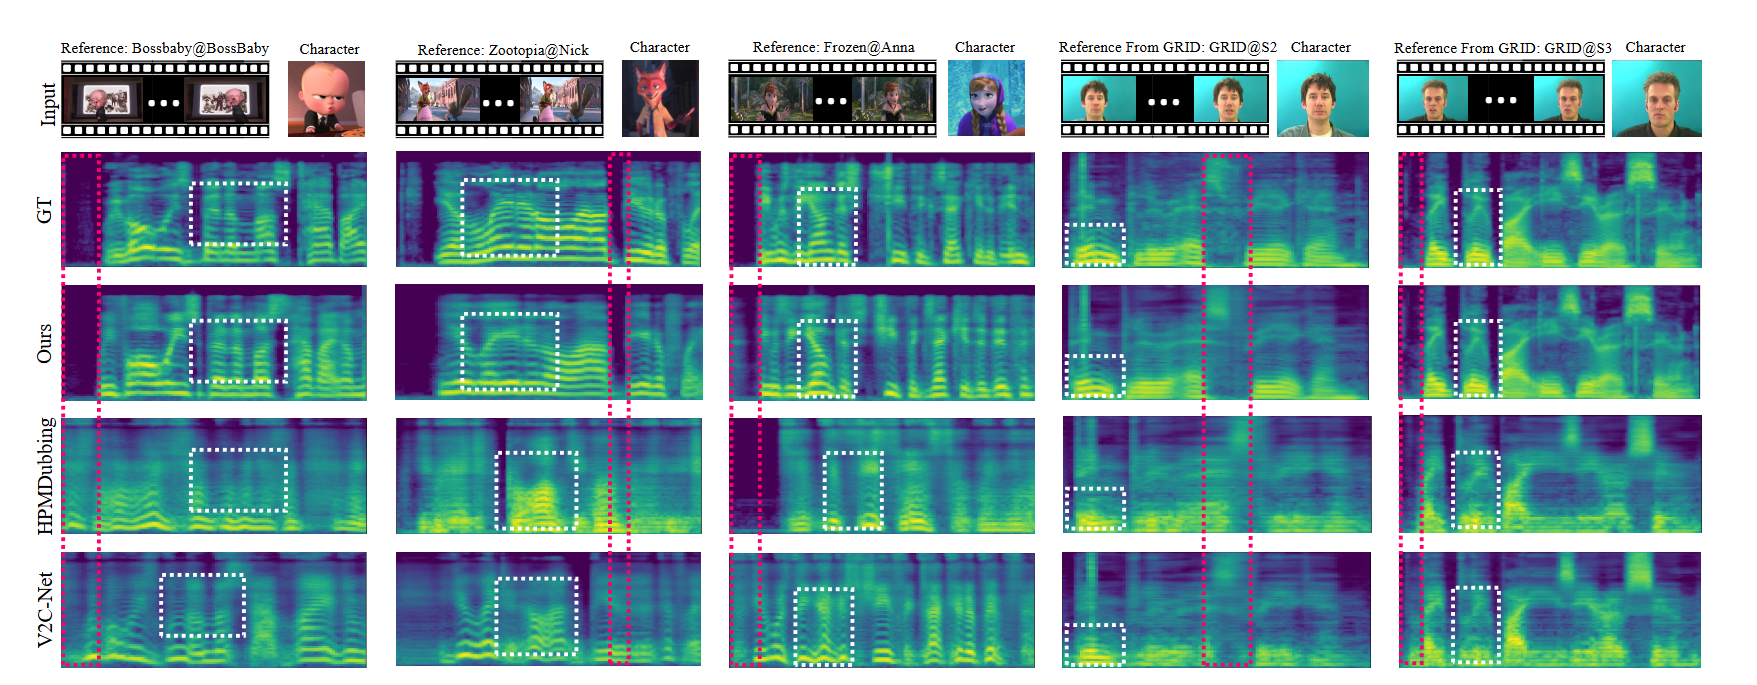
\includegraphics[width=0.6\textwidth]{figs/analysis.png} % Image path
% \caption{Comparison of Mel Spectrograms of Audio Generated by Different Models}
% \end{figure}

% \begin{itemize}
% \item \textbf{Mel Spectrogram Analysis Results:}
%     \begin{itemize}
%     \item \textcolor{red}{Red Box in Figure}: Our model outperforms others in maintaining phoneme and pause durations, especially in the V2C-Animation benchmark with complex speaking speed variations.
%     \item \textcolor{red}{White Box in Figure}: The dubbing generated by our model exhibits clearer and more natural pronunciation details, as evidenced by the clearer spectrum lines.
%     \end{itemize}
% \end{itemize}
% \end{frame}
\begin{frame}
\frametitle{Experimental Results: Qualitative Analysis of Mel Spectrograms}
\begin{figure}
\centering
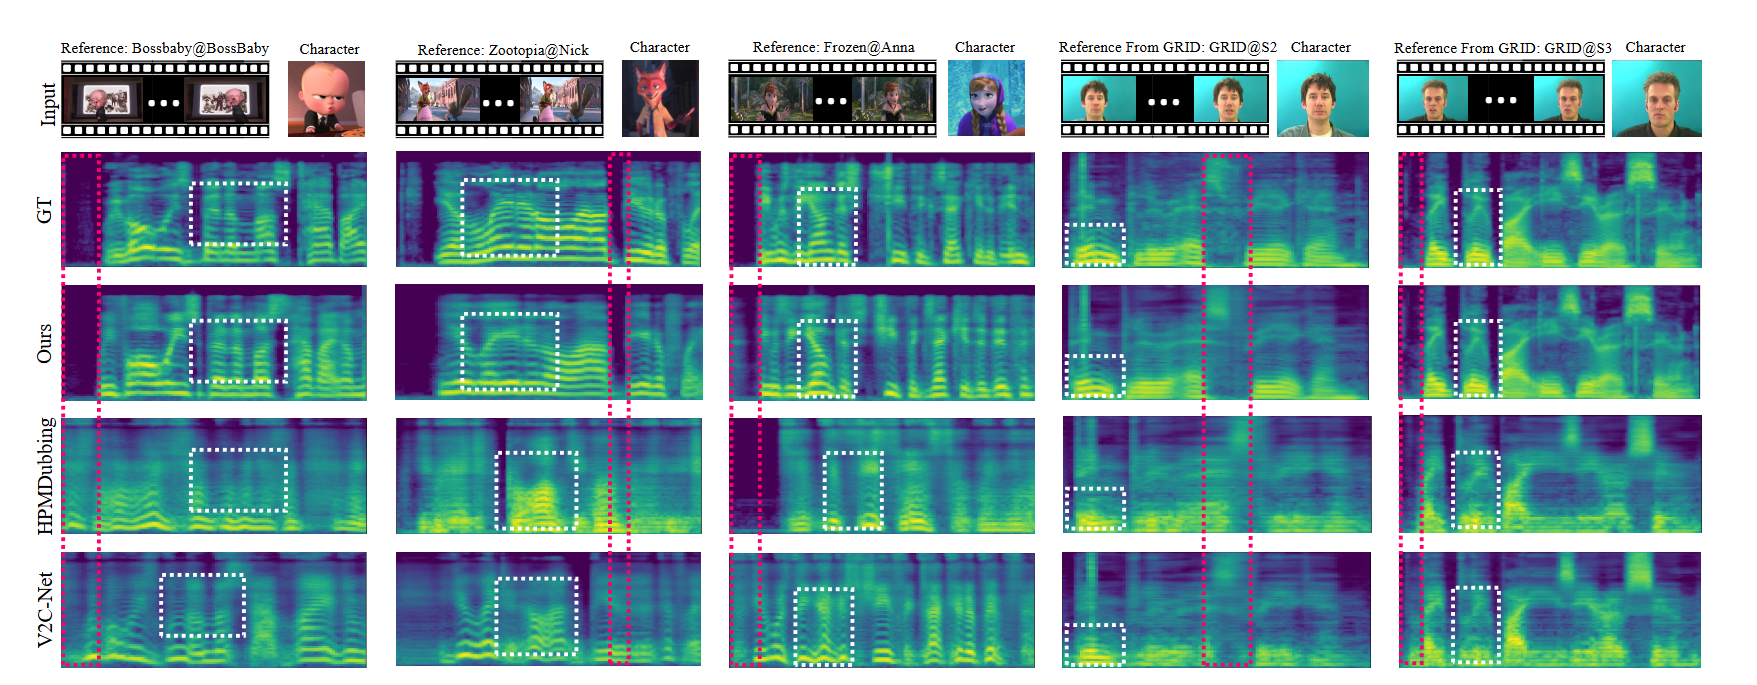
\includegraphics[width=0.6\textwidth]{figs/analysis.png} % Image path
\caption{Comparison of Mel Spectrograms of Audio Generated by Different Models}
\end{figure}

\begin{itemize}
\item \textbf{Analysis Results:}
    \begin{itemize}
    \item \textcolor{red}{Red Box}: the model better maintains phoneme and pause durations, especially in V2C-Animation benchmark.
    \item \textcolor{red}{White Box}: the model shows clearer and more natural pronunciation details.
    \end{itemize}
\end{itemize}
\end{frame}


% \begin{frame}
% \frametitle{Experimental Results: Ablation Study}
% The ablation study results fully demonstrate the necessity of each module.

% \begin{figure}
% \centering
% 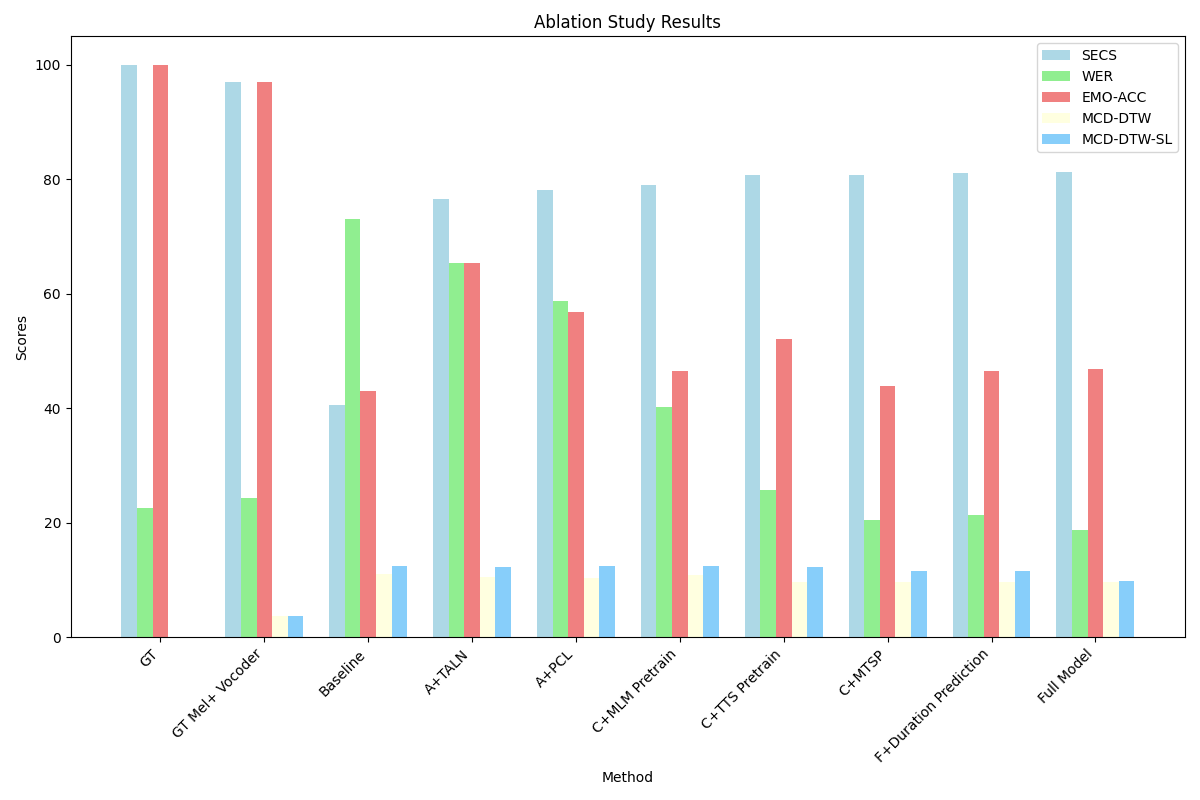
\includegraphics[width=0.4\textwidth]{figs/消融实验.png} 
% \caption{Comparison of Ablation Study Results}
% \end{figure}

% \begin{itemize}
% \item \textbf{PCL Module:} Enhances timbre cloning and emotional consistency.

% \item \textbf{MTSP Module:} Significantly reduces Word Error Rate (WER) and improves pronunciation quality.

% \item \textbf{DCR Module:} Reduces MCD-DTW-SL and enhances duration consistency.

% \end{itemize}
% \end{frame}

\begin{frame}
\frametitle{Experimental Results: Ablation Study}
The ablation study results fully demonstrate the necessity of each module.

\begin{figure}
\centering
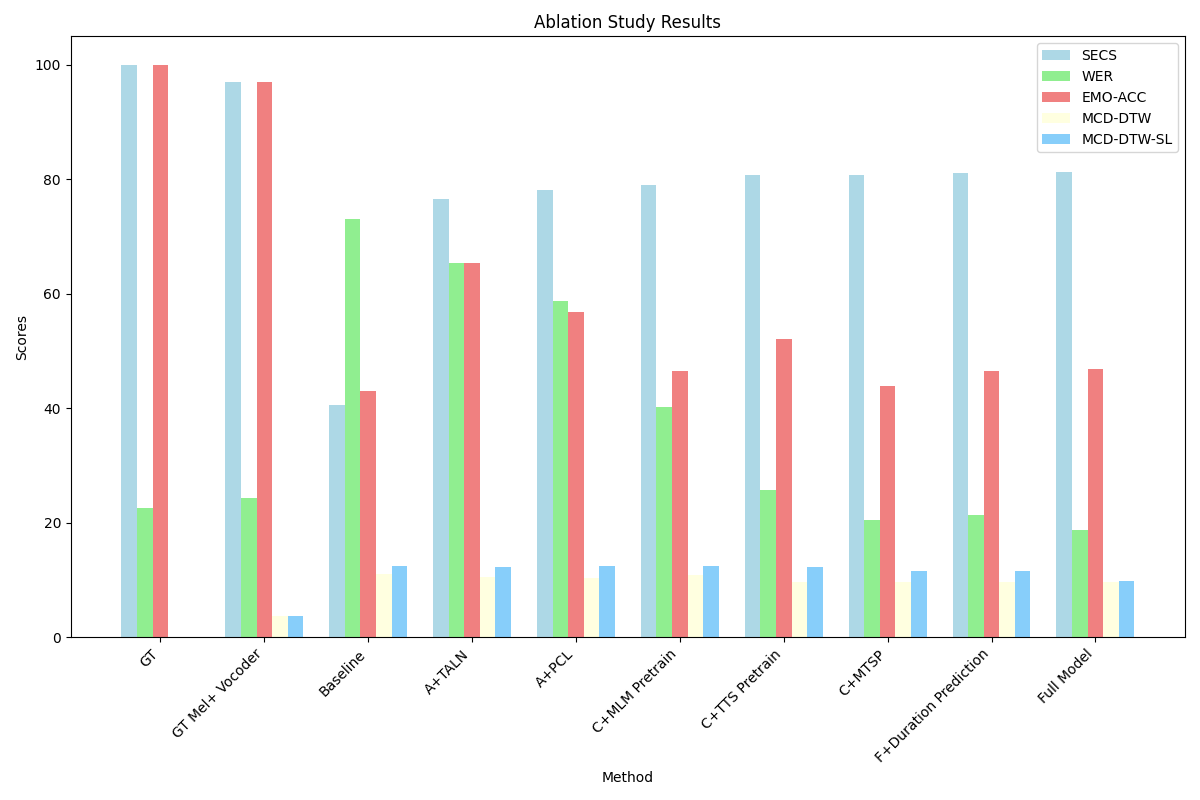
\includegraphics[width=0.4\textwidth]{figs/消融实验.png} 
\caption{Comparison of Ablation Study Results}
\end{figure}

\begin{itemize}
\item \textbf{PCL Module:} Enhances timbre cloning and emotional consistency.
\item \textbf{MTSP Module:} Reduces WER, improves pronunciation quality.
\item \textbf{DCR Module:} Reduces MCD-DTW-SL, enhances duration consistency.
\end{itemize}
\end{frame}